% \section{Objetivo}
% O objetivo deste projeto de mestrado é desenvolver técnicas de controle subótimo das juntas passivas (não atuadas) de um robô subatuado, incluindo o estudo teórico do tema, proposição de um método de controle e sua verificação
% experimental em um manipulador de três graus de liberdade \cite{Nascimento1970}.

% O teste \cite{Patagonios2001} e validação das técnicas de controle propostas foram realizados em um ambiente de simulação e no manipulador
% experimental, adquirido através do projeto FAPESP $N^{\circ}$ 98/00649-5, que se encontra em funcionamento no \gls{lasi} do Departamento de Engenharia Elétrica da USP em São Carlos. De acordo com \citeauthor{Furmento1995}, pode-se listar:
% \begin{itemize}
% \item Isso;
% \item Aquilo; e
% \item Aquele outro.
% \end{itemize}

% Então, no \gls{lasi} são realizadas as várias atividades listadas.

% \section{Motivação}
% Manipuladores mecânicos \cite{Sbornian2002} vêm sendo utilizados há várias décadas para a automação de tarefas
% repetitivas em ambientes industriais, ambientes estes de fácil acesso tanto em termos físicos quanto em termos de baixo
% risco à saúde humana. Nos últimos anos, verifica-se uma utilização cada vez maior de manipuladores em
% ambientes de difícil acesso ou inóspitos, como no interior de usinas nucleares, no fundo dos oceanos e no
% espaço. A localização dos manipuladores nesta nova gama de aplicações faz com que sua manutenção,após uma falha mecânica ou elétrica, seja custosa e demorada, portanto estes mecanismos requerem sofisticadas
% metodologias de controle tolerante a falhas \cite{ITALUS2004}.

% Após a ocorrência de uma falha em um de seus atuadores, o manipulador torna-se um sistema subatuado. Um sistema também pode se tornar subatuado quando é projetado  dessa maneira, ou quando o operador deliberadamente mantém um ou mais atuadores disponíveis inoperantes durante uma tarefa. Reduzindo o número de atuadores sem reduzir o número de graus de
% liberdade e ajustando-se o sistema de controle adequado, pode-se obter um mecanismo cujo consumo de energia é menor, mas cujas propriedades são mantidas \cite{Arystides1994}.

% \begin{figure}[ht]
% \centering
% 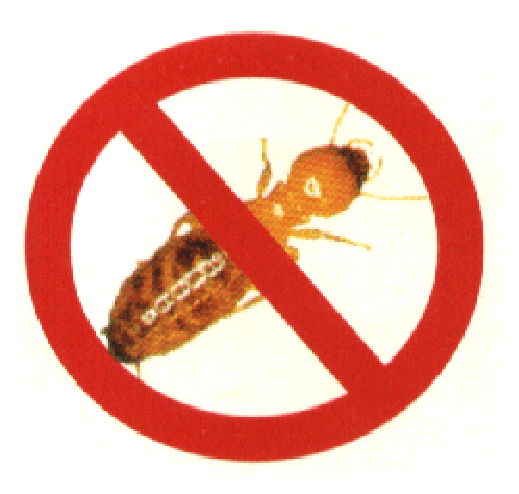
\includegraphics[width=0.5\textwidth]{Cap1/cupim}
% \caption{Proibido estacionar cupins. Legenda grande, com o objetivo de demonstrar a indentação na lista de figuras.}
% \label{cupim}
% \end{figure}

% Controle do manipulador após uma falha é fundamental do ponto de vista de operação, principalmente nos casos descritos acima, em que a localização do manipulador impede sua manutenção de forma fácil. Recentemente tem havido a combinação
% de algorítmos de detecção e isolação de falhas com os de controle pós-falha em um método unificado. Uma extensão desse trabalho, que vê o problema de controle tolerante a falhas através de uma perspectiva integrada, foi proposta por
% {marcel4}. Os autores apresentam um ambiente híbrido consistindo de três unidades básicas que garantem a compleição de tarefas na presença de qualquer número de juntas falhas (Fig.~\ref{cupim}). A primeira unidade é um esquema de detecção
% e isolação de falhas que continuamente monitora o manipulador para detectar e identificar possíveis falhas nas juntas. A segunda unidade é responsável pela reconfiguração do controle. A terceira unidade é composta de algorítmos de
% controle apropriados para cada tipo de configuração do robô, baseado na informação da unidade de reconfiguração \cite{COFFEE2000}.

% No presente trabalho nos concentramos na unidade de algorítmo de controle, e mais especificamente no problema de controle da posição  angular de uma junta falha para qualquer posição desejada de uma maneira subótima, quando dispomos
% de redundância de atuação para a realização dessa tarefa. O termo subótimo se deve ao fato de que não há garantias de otimalidade em vista das não-linearidades inerentes ao sistema e de outros fatores que serão abordados nos capítulos posteriores. Ao longo do texto, para simplificação, usaremos tanto o termo subótimo como ótimo para nos referirmos à metodologia utilizada.

% Segundo, o critério de otimização utilizado será o acoplamento entre as juntas do
% manipulador e neste caso, temos um sistema redundante quando ocorre falha de uma das juntas do manipulador de três juntas, e seu posicionamento é controlado pelas duas restantes. Nossa solução para o problema é baseada na formulação
% de redundância local, extensivamente estudada no contexto de cinemática inversa ({nakamura}). A principal contribuição deste trabalho é a extensão deste método usando as equações dinâmicas de manipuladores subatuados e a utilização do índice de acoplamento como um critério para a minimização do torque e da energia gasta pelo sistema durante o controle das juntas falhas.

% \begin{figure}[ht!]
% \centering
% 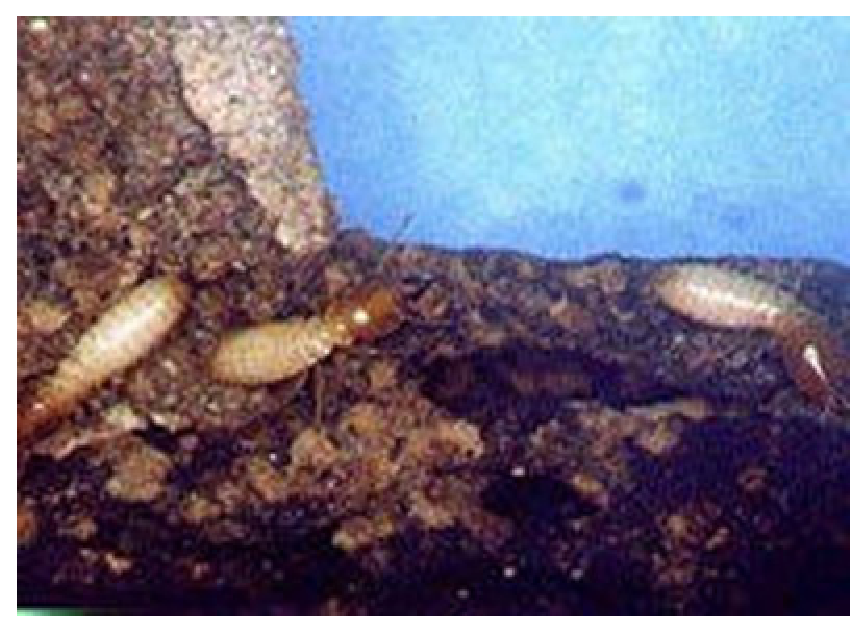
\includegraphics[width=1\textwidth]{Cap1/cupimconcreto}
% \caption{Exemplo real de cupim frente ao seu dilema.}
% \label{FDII}
% \end{figure}

% \section{Organização do trabalho}
% \subsection{Sub-organização}
% O capítulo 1 contém a introdução do trabalho, onde são expostos o objetivo, a motivação do mesmo, a descrição do sistema e a formulação do problema com a nomenclatura utilizada; além de uma revisão bibliográfica da literatura relacionada ao tema do trabalho.

% \subsubsection{SubSub-organização}

% No capítulo 2 apresentamos a modelagem dinâmica de um manipulador subatuado e o conceito de índice de acoplamento para medir o acoplamento dinâmico entre as juntas ativas e passivas. Este índice é utilizado para a análise e projeto de uma metodologia de controle subótimo do manipulador.

% \subsubsection{Outra subsub-organizacao}

% O capítulo 3 apresenta o controle subótimo de manipuladores através de redundância de atuação. Descreve-se a técnica de controle ponto a ponto de manipuladores subatuados. A seguir mostramos  a linearização destes por realimentação, cujo efeito é linearizar e desacoplar o sistema não linear. Finalmente é proposta uma sequência de controle subótimo local das juntas passivas visando a minimização de certos critérios como torque, velocidade e em particular a energia consumida pelo sistema. Este é de fato o tema principal deste mestrado.

% É também apresentado no capítulo 4 um resumo do projeto de controladores  $H_{2}$ e $H_{\infty}$, cuja principal vantagem é a robustez na presença de incertezas paramétricas e distúrbios externos.

% O capítulo 5 mostra as características e a operação do robô e do ambiente de simulação utilizados nos testes e experimentação da metodologia apresentada.

% Os procedimentos da metodologia e os resultados obtidos para algumas configurações e diferentes controladores encontram-se no capítulo 6.

% No capítulo 7 são apresentadas as conclusões do trabalho.

% Quatro apêndices fazem parte do trabalho. O apêndice A apresenta alguns tópicos de álgebra linear que são a base do método proposto. No apêndice B são mostradas as equações da matriz de inércia e do vetor de torques não-inerciais
% utilizados na modelagem dinâmica do manipulador. No apêndice C temos as expressões literais dessas equações feitas no software MAPLE e no apêndice D alguns programas feitos no software MATLAB utilizados no projeto \cite{Furmento1995, Morgado2003}.


% \subsection{Como utilizar o glossário}
% O glossário no \LaTeX é automatico, utilizando o pacote ``glossaries'', então basta adicionar as entradas em ``listaabreviaturas.tex'' e em ``listasimbolos.tex'' e utilizar o comando ``$\backslash$gls\{\}''.
% A lista de abreviaturas e de simbolos será gerada automaticamente de acordo com os elementos que foram utilizados no texto.

% A primeira vez que uma abreviatura é chamada é automaticamente representada em sua forma completa: \gls{ctq}.
% Ao utilizar o comando depois da primeira vez, apenas a abreviatura será utilizada: \gls{ctq}.

% O glossário também pode ser utilizado para simbolos matemáticos, então pode-se definir por exemplo uma variável delta de Kronecker e utilizar o comando ``$\backslash$gls\{\}'', \gls{delta_kro}. 
% Se houver a necessidade de modificar o simbolo utilizado, não precisa alterar todas as entradas ao longo da tese, basta alterar o simbolo em ``listadesimbolos.tex''.


